%! TEX root = main.tex  %
\documentclass[main.tex]{subfiles} % Wichtig!

\begin{document}

\subsection{Projektmanagement}
Das Projektmanagement spielt eine zentrale Rolle in der Vorbereitungsphase der Bachelorarbeit 
und bildet die Grundlage für den Erfolg des gesamten Vorhabens. Dabei geht es nicht nur um die 
reine Planung, sondern auch um eine effiziente Steuerung und kontinuierliche Kontrolle aller 
Arbeitspakete und derer Ergebnisse. Die besondere Herausforderung der Arbeit liegt darin, 
das umfangreiche Themengebiet, das für diese Bachelorarbeit relevant ist, innerhalb des engen 
Zeitrahmens von 14 Wochen sinnvoll und fundiert zu bearbeiten. Das Themengebiet umfasst diverse 
Bereiche der Informatik. Darunter fallen Audioverarbeitung, maschinelles Lernen, 
Softwareentwicklung und auch einiges an mathematischem Hintergrundwissen. Daher wurde ein 
klassisches Vorgehensmodell gewählt. Dies bedeutet, dass sowohl die Planung als auch die Umsetzung 
in klar definierte Arbeitspakete unterteilt sind. 

\newpage
\subsubsection{Produkt Backlog}

Der Product Backlog besteht primär aus den Arbeitspaketen, die in der Grobplanung definiert werden.
Gewisse Arbeitspakete nehmen mehr Zeit in Anspruch als andere und erstrecken sich über mehrere
Semesterwochen. Die Arbeitspakete werden in der Tabelle \ref{fig:backlog_table} aufgeführt.


\begin{table}[ht]
    \centering
    \begin{tabularx}{\textwidth}{llX}
    \toprule
    \textbf{Phase} & \textbf{Semesterwoche} & \textbf{Beschreibung des Arbeitspakets} \\
    \midrule
    Stand der Forschung     & SW1/2  & Setup (git, tes, usw.) \\
                            & SW2    & Siri research  \\
                            & SW2/3  & Marktanlyse \\
                            & SW3    & Audio Allg., Audio API \\
                            & SW3/4  & Fourier Transform, Spektrogramm \\
    \addlinespace
    Erstellung des Modells  & SW4/5  & DNN \\
                            & SW4/6  & Collect Data "Hey FOOBY" \\
                            & SW5    & RNNs verstehen \\
                            & SW5/6  & Privacy und Ethik,  \\
                            & SW5/6  & Datasets 'other' evaluation \\
                            & SW6/7  & Training \\
                            & SW7/8  & Evaluation \\
    \addlinespace
    Prototype               & SW9       & PyTorch Mobile integration \\ 
                            & SW10/11   & Mobile Demo App Entwicklung \\
                            & SW12      & Video für Bachelorarbeit \\
                            & SW11/12   & Feedback der App sammeln \\
                            & SW12/14   & Dokumentation fertigstellen \\

    \bottomrule
    \end{tabularx}
    \caption{Hierarchische Auflistung der Arbeitspakete}
    \label{fig:backlog_table}
\end{table}



\subsubsection{Risikomanagement}
Als mögliche Risiken wurden im Projekt zum einen die Komplexität des Themas und zum anderen die
begrenzte Zeit für die Bearbeitung identifiziert. Weitere Risiken, die während der 
Projektdurchführung aufgetreten sind, werden nachfolgend zusammengefasst. Die Tabelle 
\ref{tab:risiken} zeigt die identifizierten Risiken, deren Eintrittswahrscheinlichkeit sowie die 
Auswirkung auf das Projekt.

\begin{table}[h]
    \centering
    \begin{tabular}{|l|c|c|}
        \hline
        \textbf{Risiko} & \textbf{Eintrittswahrscheinlichkeit} & \textbf{Auswirkung} \\
        \hline
        Komplexität des Themas & Hoch & Gross \\
        \hline
        Begrenzte Zeit für Bearbeitung (14 Wochen) & Mittel & Kritisch \\
        \hline
        80\% Arbeitspensum, 20h pro Woche am Wochenende & Hoch & Mittel \\
        \hline
        Grosser Release in aktueller Arbeit bis Ende Oktober & Hoch & Hoch \\
        \hline
        Qualität des Speech Recognizers & Mittel & Kritisch \\
        \hline
        Latenz und Performance des Erkenners & Hoch & Gross \\
        \hline
    \end{tabular}
    \caption{Identifizierte Risiken im Projekt}
    \label{tab:risiken}
\end{table}



\begin{landscape}
    \subsection{Grobplanung}
    Die Grobplanung zeigt die wichtigsten Meilensteine sowie die anfängliche zeitliche Einteilung 
    der einzelnen Themenbereiche die für die Bachelorarbeit relevant sind, aufgezeigt. Die
    Grobplanung ist in Abbildung \ref{fig:grobplanung} dargestellt.

    \begin{figure}[!htb]
        \centering
        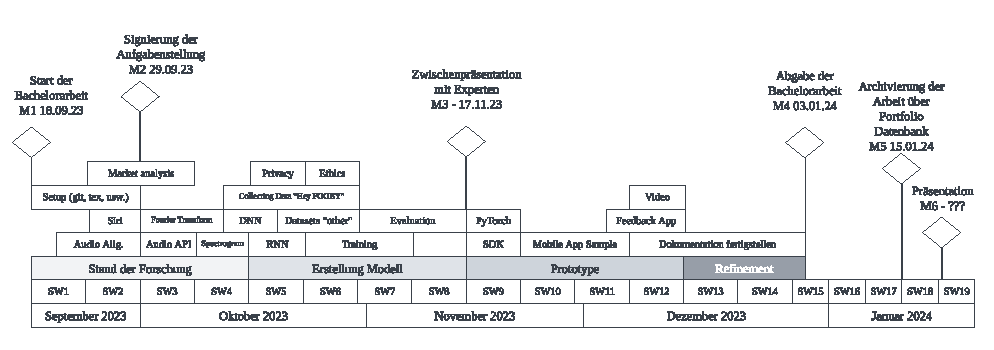
\includegraphics[width=\linewidth]{img/projectplan.pdf}
        \caption{Grobplanung}
        \label{fig:grobplanung}
    \end{figure}
\end{landscape}



\end{document}
